\documentclass{standalone}
\begin{document}
\section{Chapter 2 Human Factors}
\begin{itemize}
	\item The goal is to stimulate all perception channels in such a way that the user feels completely immersed in the virtual environment and accepts it as real.
	\item we are forced by our senses to perceive every environment in the sameway, nomatter wheter this environment is real or virtual
	\item visual, accoustic thermal, haptic and olfactory perception($80 \%$ of the overall information is perceived via the visual channel)
	\item Human Perception
	\begin{itemize}
		\item Perception
		\begin{itemize}
			\item Sensous physiology: the perception of stimuli, performed by sensory cells or by sensory organs.
			\item Psychology : Process of sensuous perception of an object without any conscious identification of the perceived object.
		\end{itemize}
		\item Cognition
		\begin{itemize}
			\item Psychology : Collective name for all processes or structures that are involved in the cognition process. e.g. imagination, estimation, mnemory, rememberance, learning. etc
		\end{itemize}
	\end{itemize}
	\item Four elementary attributes of stimulus
	\begin{itemize}
		\item modality: quality of a stimulus(the type of physical energy that is responsible for the stimulus)
		\item intensity: The strength of a stimulus defines the intensity of a sensation(below a specific threshold, the stimulus is not detected
		\item duration: relationship between the intensity of the stimulus and the duration of the sensation defines the perceived intensity
		\item location: The ability to locate the position of a stimulus and the ability to distinguish between two spatially close stimuli are important measures of the awareness of the spatial distribution of a sensory experience
	\end{itemize}
	\item action potential: Only if the intensity is larger than a particular threshold, an electrical discharge is generated by the responsible receptors
	\item only the sensory part of the cognition process can be addressed by devices of the virtual environment. (Figure)
\end{itemize}
\begin{figure}[H]
\centering
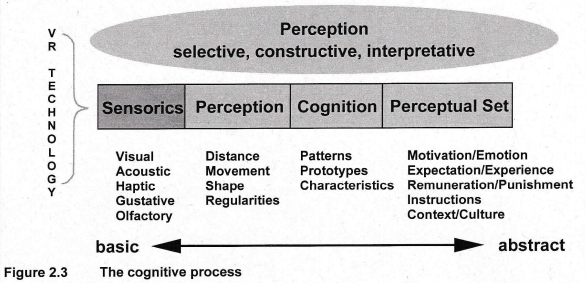
\includegraphics[width = 0.7\linewidth]{Figures/2_3.png}
\end{figure}
\subsection{The Human Eye}
\subsubsection{Viewing Angle}
\begin{itemize}
	\item Field of view characterized by: optical setup of the eye / the position of the eye in the face
	\item although field of view is very large perception of sharp images only possible in much smaller area
	\item viewing cones of both eyes overlap in a reange of approximately 120 degrees
	\item Four opening angles of the field of view
\begin{table}[H]
\centering
\begin{tabular}{|l|c|c|r|}
\hline
 nasal & temporal & superior & inferior \\ \hline
60 deg & 100 deg & 60 deg & 70 deg \\ \hline
\end{tabular}
\end{table}
\end{itemize}
\subsubsection{Temporal Resolution}
\begin{itemize}
	\item pupil can adapt to changing light conditions with a maximum frequency of 4 Hz	
	\item flicker consolidation frequency: maximum possible frequency without noticing any flickering
	\item perception of flickering not only depends on brightness but also the size of field of view and the location of light source it the FOV
\end{itemize}
\subsubsection{Accommodation and Convergence}
\begin{itemize}
	\item eye focuses onto shortest possible distance until object is visible: needs edges, patterns or contrours to focus: In compelte darkness, the eye cannot focus anymore
	\item results in near sightedness when looking through a optical device
	\item depth estimation up to 10 meters is made with stereoscopic vision $$ tan \frac{\epsilon}{2} = \frac{a}{2} \frac{1}{e}$$
\end{itemize}
\subsubsection{B/W Perception, Color Perception}
\begin{itemize}
	\item light models: wave-model is more sufficient regarding the light as a electromagnetic radiation with a wavelength between 380 nm and 780 nm
	\item color perception is done by a single eye
	\item color is perceived using special receptors on the retina
	\begin{itemize}
		\item sticks : only measure the intensity of the incoming light(Black and White). used at night but easily saturated.(more sensitive than uvulas)
		\item uvulas : used in daylight(light at night are not sufficient to work for uvulas), different uvulas for each color : (blue-sensitive uvulas 4 \% at 430nm , green-sensitive uvulas 32 \% at 530 nm, red sensitive uvulas 64 \% at 560 nm)
		\item 95 \% are sticks and 5 \% are color sensitive uvulas
	\end{itemize}
	\item colors are coded into three basic colors, then two difference channels (red - green), (blue - yellow). addition of all colors result in the non-colored brightness.
		\begin{figure}[H]
			\centering
			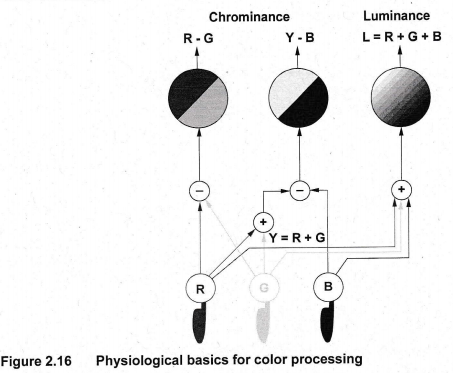
\includegraphics[width = 0.5\linewidth]{Figures/2_16.png}
		\end{figure}
\item During daylight: different kind of uvulas capture the basic colors red, green and blue while the sticks only measure brightness
\item During darkness: uvulas do not provide any color information, but only black(black does give any information to the brain?), small amount of light is sufficient to activate the sticks without saturating them
\item hue, saturation, brightness imitate the human color perception
\item there is also a contrast amplification in oerder to increase the perceived sharpness of the image
\item focal length depends on the color(Chromosteropsis: if more colors exist at the same distance, the eye can only focus on them, if red, blue exist the eye will focus on the red field due to the larger amount of red sensitive receptors)
\end{itemize}
\subsubsection*{Color Models}
\begin{itemize}
		\item CIE color model(Commission Internationale del'Eclairage): based on the typical sensitivity of the different uvulas(perception oriented color model)
		\item YUV color model: Takes into account the high green sensitivity into account, while sensitivity to red and blue is significantly lower(perception oriented color model)
		\begin{equation}
		\begin{split}
		C_b = B - Y \quad color \quad  difference \quad signal \quad 1 \\
		C_r = R - Y \quad color \quad difference \quad signal \quad 2 \\
		Y brightness (luminance)
		\end{split}
		\end{equation}
		\item RGB color model: does not take the physiology of the human eye into account(technical color model), basic colors are scaled to 1 and define a coordinate system
		\item CMY color model: is used by objects that do not emit light themselves, color used by printers
		\item HSV color model(also HSB): Defined by hue, saturation, value. In this color model, colors are arranged in a circle around the vertical axis
\end{itemize}
\subsubsection{Three-dimensional Viewing}
\subsubsection*{Spatial Viewing}
\begin{itemize}
\item spatial viewing can be performed with only one eye and thus is also called monocular viewing(only psychological aspects are considered)
	\begin{itemize}
		\item Size of the Image on the Retina: If the real size is known, the brain compares the perceived size with the real size stored in the brain and calculates information of the position and the distance of the object
		\item Resoultion of the Perceived Image: Objects with blurred surface appear far away
		\item Overlap: If one object is in front of the other it has to be closer to the spectator than the object
		\item perspective: Far objects appear smaller than close ones
		\item shaded objects and shadows: I the light source is know, the object that causes the shadow appears closer to the light source
		\item textures: A spatial effect also appears when mapping textures perspectively onto an object. Wrong selection of textures could completely camouflage the geometry or pretend a wrong geometry
		\item motion parallax: the farther away an object is, the slower it moves on the retina when moving relatively to the user
	\end{itemize}
	\item Perception Rules Depending on geometry
	\begin{itemize}
		\item Rules of proximity: Spatially or temporally neighboring elements are perceived to belong together and to be part of the same element
		\begin{figure}[H]
			\centering
			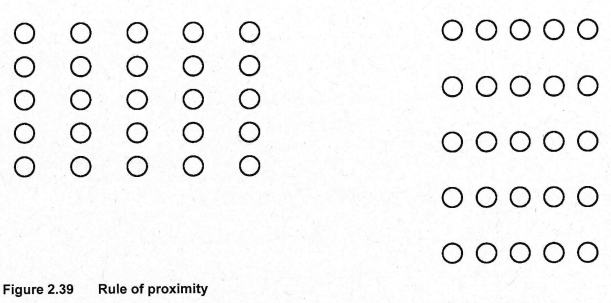
\includegraphics[width = 0.5\linewidth]{Figures/2_39.png}
		\end{figure}
		\item rule of similarity/rule of identity: Similar or identical objects appear coherently 
		\begin{figure}[H]
			\centering
			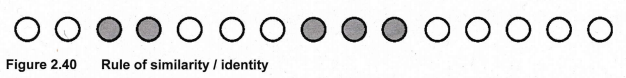
\includegraphics[width = 0.5\linewidth]{Figures/2_40.png}
		\end{figure}
		\item identity versus proximity: effects can be amplified or reduced
		\begin{figure}[H]
			\centering
			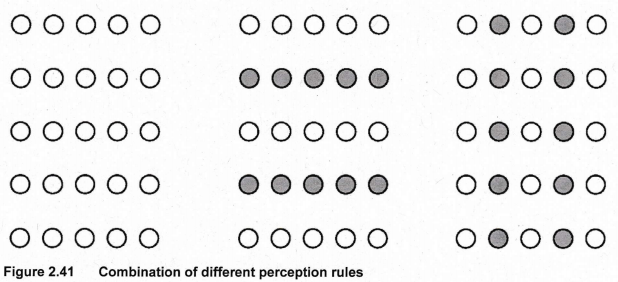
\includegraphics[width = 0.5\linewidth]{Figures/2_41.png}
		\end{figure}
		\item rule of harmonic continuation: elements that are spatially or temporally arranged in a simple harmonic or well defined order appear coherently and thus belong to the same geometric figure
		\begin{figure}[H]
			\centering
			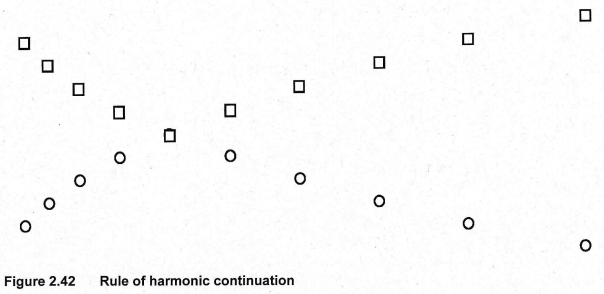
\includegraphics[width = 0.5\linewidth]{Figures/2_42.png}
		\end{figure}
		\item rule of closed lines: Contours, which are not completely closed, will be automatically closed during the perception process
			\begin{figure}[H]
				\centering
				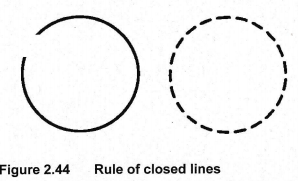
\includegraphics[width = 0.5\linewidth]{Figures/2_44.png}
				\end{figure}
		\item rule of symmetry: if none of the mentioned rules could be applied, the space between symmetric contours shapes a figure, rather than the space between asymmetric contours
			\begin{figure}[H]
				\centering
				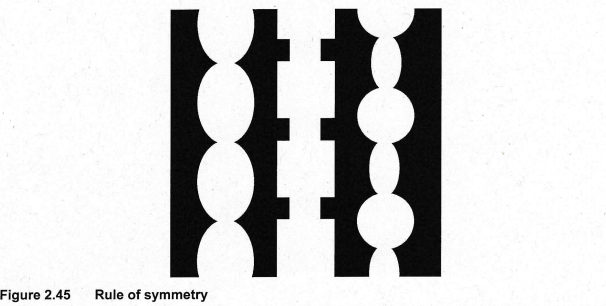
\includegraphics[width = 0.5\linewidth]{Figures/2_45.png}
			\end{figure}
		\item the principle of harmonic shape: The structure will be perceived, that has as many simple figures as possible
			\begin{figure}[H]
			\centering
			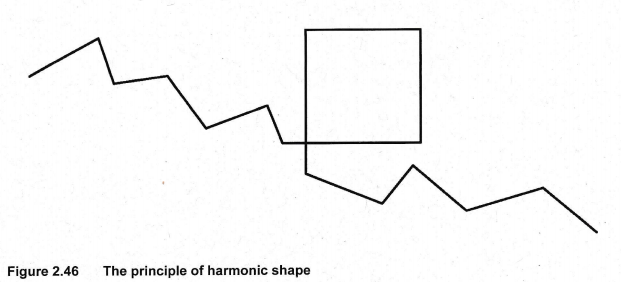
\includegraphics[width = 0.5\linewidth]{Figures/2_46.png}
			\end{figure}
		\item contours: 
			\begin{figure}[H]
			\centering
			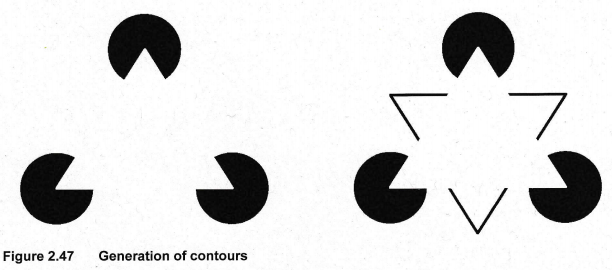
\includegraphics[width = 0.7\linewidth]{Figures/2_47.png}
			\end{figure}
	\end{itemize}
\end{itemize}
\subsubsection*{Allocation Problems}
\begin{itemize}
	\item wrong perspective, brightness of objects given context, comparison with known patterns
	\item peripheral drift illusion: depends on difference in brightness or color(static images seem to move when viewing at different areas of the image), illusion of movement is always from black to dark gray or white to a light gray
	\item The reason for allocation problem is the fact that the interpretation of the perceived impression is done in different parts of the brain
	\item Hermann grid: width of the white lines corresponds to the diameter of the receptive fields on the retina(contrast amplification by ON-center neurons, OFF-center neurons)
		\begin{figure}[H]
			\centering
			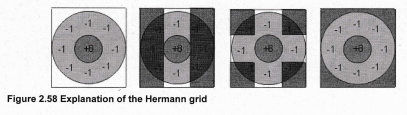
\includegraphics[width = 0.7\linewidth]{Figures/2_58.png}
		\end{figure}
		\item scintillating grid: consists of a herman grid with gray lines on a black background, with white dots on the crossing(effect: outside the zone of interest, black dots appear instead of original white dots)
		\begin{figure}[H]
			\centering
			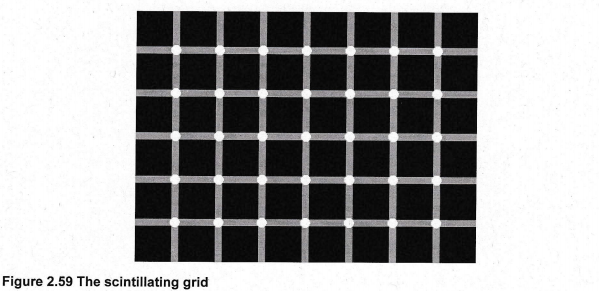
\includegraphics[width = 0.7\linewidth]{Figures/2_59.png}
		\end{figure}
		\item barber's pole effect: rotating cylinder with spiral(motion is always in direction of the aperture's longest edge)
\end{itemize}
\subsubsection*{Stereoscopic viewing}
\begin{itemize}
	\item In order to focus both eyes on the object, they are directed onto the object. THis will result in a convergence angle between the optical axes of both eyes	
	\item The point is projected on non-corresponding areas on the retina on both eyes. This gives a spatcial impression
\end{itemize}
\subsubsection{Conflicts between Virtual Reality and the Physiological and Psychological Visual Perception}
\begin{itemize}
	\item Since all virtual objects are visible on the projection plane, the human eye does not have to perform an accommodation anymore, but only focuses once on the given distance between the user and the projection plane
	\item psychological apsects are also not fulfilled
\end{itemize}
\subsection{The Human Ear}
\begin{itemize}
	\item Functionality of hearing
	\item Sound signals and sound sources
	\item Location of sound sources
	\item sensitivity and loudness(very important psychological factor)
	\item When simulating objects in virtual environments, the acoustical sensation is very important
\end{itemize}
\subsubsection{Spatial Hearing}
Spatial hearing desribes the accoustical determination of a sound source's position in a room. Two princilples:
\begin{itemize}
	\item monaural hearing
	\begin{itemize}
		\item Using one ear only: very rough localization($\pm 20 \deg deviation from correct localization$) : does not play important role
	\end{itemize}
	\item binaural hearing
	\begin{itemize}
		\item difference in intensity: only possible if wavelength of the sound is small compared to the size of the head
		\item difference in runtime: brain capable of detect runtime differences of approximately 30us
		\item can calculate the run time difference:
		$$
		\Delta x = d sin \alpha \\
		\Delta t = \frac{\Delta x}{c} = \frac{d}{c} sin \alpha \quad c = 340m/s
		$$
	\end{itemize}
	\begin{figure}[H]
			\centering
			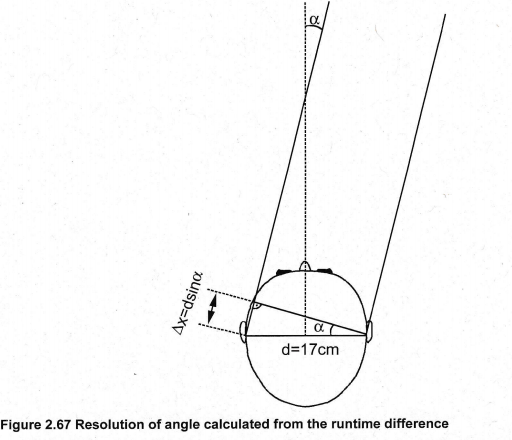
\includegraphics[width = 0.7\linewidth]{Figures/2_67.png}
		\end{figure}
	\item Allocation Problems of the ear
			\begin{itemize}
			\item Shephard effect: simulates increasing melody to the user although the pitch stays constant all the time
		\end{itemize}
\end{itemize}
\subsection{The Haptic Channel}
\subsubsection{The Human Information Flow}
\begin{itemize}
	\item the entirety of all perceptions through the sense of touch
	\item about 80 \% of all information is perceived by the visual sense, other 15 \% by the auditory sense. The remaining 5 \% are fr the haptic and olfactoric sense. 
\end{itemize}
\subsubsection{The Haptic Perception}
\begin{itemize}
	\item The haptic takes place all over the body, thus it is impossible to generate a complete simulation in the haptic field: The human hand is the most relevant element in the field of haptics
	\item well known input device: mouse and keyboard provide haptic feedback addition to acoustic feedback.
	\item required for teleoperation
	\item Using the had to perform a manipulation
	\begin{itemize}
		\item Contact Phase: Describes the first contact of the fingers with an object(felt 200 ms after contact)
		\item Grasping Phase: has the largest flexibility and interactability
		- Grasping for increased power / Grasping with increased dexterity
		\item Touching Phase: For characterizing the properties of objects, different hand-object interactions are needed
	\end{itemize}
	\item Grasping can be seperated with thwo fields
	\begin{itemize}
		\item grasping with increased power
		\item grasping with increased dexterity
	\end{itemize}
	\item Haptic desribes the influence of foces of any kind onto the human body(tactile propriorceptive, kinesthetic)
	\begin{itemize}
		\item tactile: using perception cells in the skin(pressure, temperature, vibration)
		\item propriorceptive: Influence of force caused by the weight of the object onto the sensors in the musculature
		\item kinesthetic sensation is the perception of acceleration forces onto the body 
	\end{itemize}
	\item some haptic information can be directly processed in the skin nearby the sensor(reflex reaction allows much faster reaction)
\end{itemize}
\subsubsection*{Basics on the Physiology of the Senses in the Skin}
\begin{itemize}
	\item Skin registers pressure, touch, vibration (=sense of touch), temperature and pain. This surface sensibility (together with the depth sensibility (muscle, joint and string receptors)) is also called somatovisceral sensibility
	\begin{figure}[H]
			\centering
			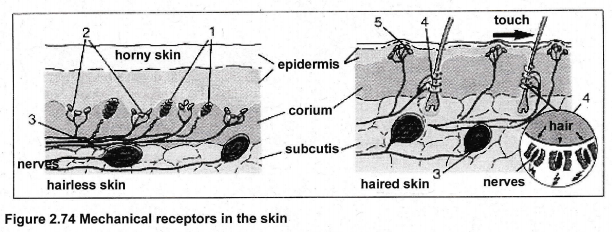
\includegraphics[width = 0.7\linewidth]{Figures/2_74.png}
	\end{figure}
	\begin{itemize}
		\item Meissner corpuscles(Fig.2.74->1): rapidly adapting receptors, provide information about the movement across the skin and thus velocity
		\item Merkel's Disks: slowly adapting receptors, react on pressure stimuli and provide information about vibrations
		\item Pacininan corpuscles(Fig.2.74->3): rapidly adapting receptors, sense acceleration as well as light touch and vibrations
		\item Raffini corpuscles detect pressure and skin shear as well as thermal changes
		\item Hair-root plexus(Fig.2.74->4) also called follicle, principle mechanoreceptor detects any movement on the skin surface
		\item Meissner cells(Fig.2.74->1) and hair receptors(Fig.2.74->4): detect the touch.(Not the intensity is important(bending of the hair) but the speed by the sensation changes.
		\item Pacini cells(Fig.2.74->3) specialized to detect vibrations
	\end{itemize}
	\item receptors can be divided into slowly adapting and rapdily apdapting mechanoreceptors
	\begin{itemize}
		\item rapidly adapting receptors respond to onset and often also termination but not throughout during stimulus-> sensorial adaptation
	\end{itemize}
	\item receptors can be classified by spatial resolution and temporal resolution
	\begin{itemize}
		\item intensity receptors: P-receptors
		\item speed receptors: D-receptors
		\item PD receptors are a mixture, which measure for example the position of the joints
	\end{itemize}
	\item Thermo receptors exist for a temperature range below 36 degrees(cold receptors) and for a temperature range above 36 degrees(heat receptors)
\end{itemize}
	\begin{figure}[H]
			\centering
			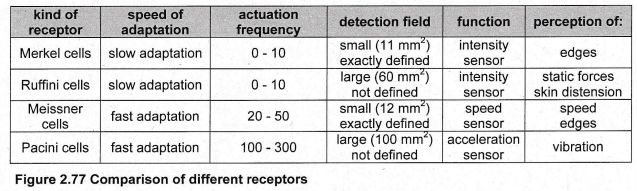
\includegraphics[width = 0.7\linewidth]{Figures/2_77.png}
	\end{figure}
\subsection{The collaboration of all Senses}
\begin{itemize}
	\item conscious and unconscious perception can be described using the so-called inner model
	\begin{itemize}
		\item Describes the context between the performed action and the expected sensor information
		\item the inner model contains the expected values of the receptors for the performed action
	\end{itemize}
	\item Pushing a button example
	\begin{figure}[H]
			\centering
			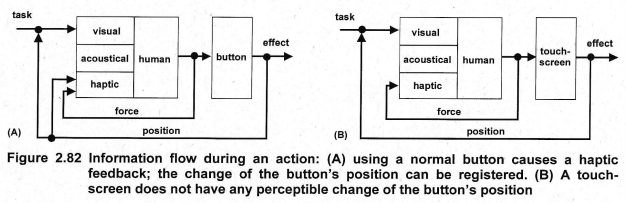
\includegraphics[width = 0.7\linewidth]{Figures/2_82.png}
	\end{figure}
	\item McGurk effect: If acoustic and visual stimuli are not correlated
\end{itemize}
\end{document}